\documentclass[Main]{subfiles}

\begin{document}

\section{A symmetric erasure and error channel has channel model
given in Figure 1}
\begin{figure}[H]
\centering
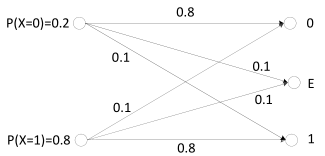
\includegraphics[width=0.4 \textwidth]{Last1}
\caption{ A symmetric erasure and error channel.}
\end{figure}


\paragraph{1. Calculate the source entropy $H(X)$.}

Source entropy, $H(x)$, in bits pr. symbol:
\begin{align}
H(x) &= P(0) log_2\bigg(\dfrac{1}{P(0)}\bigg) + P(1) log_2\bigg(\dfrac{1}{P(1)}\bigg)\\
	&= 0.2 log_2\bigg(\dfrac{1}{0.2}\bigg) + 0.8 log_2\bigg(\dfrac{1}{0.8}\bigg)\\
	&= 0.7219 \dfrac{bits}{symbol}
\end{align}
I can also be calculated in Matlab as in \codeTitle \ref{lst:Hx}

\begin{lstlisting}[caption=Source entropy, style=Code-Matlab, label=lst:Hx]
A = [0.2 ; 0.8];
B = [0.8 0.1 0.1 ; 0.1 0.1 0.8];

%Entropy, H(X)
Hx = 0;
for i = 1:size(A,1)
    Hx = Hx + (A(i,1) * log2(1 / A(i,1)));
end
Hx 
\end{lstlisting}
\code{Hx = 0.7219}
\\
\\
\paragraph{2.  Calculate the output entropy H(Y)}
To calculate the output entropy the following applies:
\begin{align}
H(Y) &= \sum_j P(y_j)log_2 \dfrac{1}{P(y_j)}
\end{align}

This can be calculated in \texttt{Matlab} as in \codeTitle \ref{lst:1step2}

\begin{lstlisting}[caption=H(Y), style=Code-Matlab, label=lst:1step2]
A = [0.2 ; 0.8];
B = [0.8 0.1 0.1 ; 0.1 0.1 0.8];

%H(Y)
HY = Hy(A, B)
\end{lstlisting}
\code{HY = 1.222}
\\
\\
The function \texttt{Hy(A,B)} is defined in \codeTitle \ref{lst:Hy}

\begin{lstlisting}[caption=Output entropy -- H(Y), style=Code-Matlab, label=lst:Hy]
function res = Hy(A, B)
% Output entropy, H(Y)
% H(Y) = P(y_1)*log2(1/P(y_1)) + ... + P(y_n)*log2(1/P(y_n))
% A = P(X) (all values)
% B = Channel describtion

val = 0;
for i = 0:length(B(1,:))-1
    val = val + Py(A, B, i) * log2(1/Py(A, B, i));
end
res = val;
end
\end{lstlisting}
$P(Y)$ can be calculated as 
\begin{align}
P(Y) &= \sum_{i=1}^u P_{i1} \cdot P(x_i)
\end{align}
and with \codeTitle \ref{lst:Py}

\begin{lstlisting}[caption=P(Y), style=Code-Matlab, label=lst:Py]
function res = Py(A, B, y)
% A = P(X) (all values)
% B = Channel description
% y = Which y to be calculated
% P(Y) = P_11 * P(x_1) + P_21 * P(x_2) +...+ P_u1 * P(x_u)
% Probability that a given symbol is present at the channel output

    value = 0;
    for i = 1:length(A(:))
        value = value + B(i, y+1)*A(i);
    end
    
    res = value;
end
\end{lstlisting}










\paragraph{3. Calculate the mutual information $I(X,Y)$.}
The mutual information can be calculated as:
\begin{align}
H(y) &= \sum_j P(y_i)log_2 \dfrac{1}{P(y_j)}\\
%	&= 0.9341\\
H(y,x) &= \sum_{i,j} P(x_i, y_i)log_2\dfrac{1}{P(y_j/x_i)}\\
I(x,y) &= H(y) - H(y,x)	
%ChannelCapacity &= H_{max}(Y)- H(y/x)\\
%	&= 0.1887
\end{align}




\begin{lstlisting}[caption=Mutual information, style=Code-Matlab, label=lst:Mutual]
A = [0.2 ; 0.8];
B = [0.75 0.25 ; 0.25 0.75];

% H(Y/X)
HYX = Equivocation(A, B);

% H(Y)
HY = Hy(A, B);

% Mutal information, I(X/Y)
IXY = HY - HYX

\end{lstlisting}
\begin{align}
H(Y/X) &= 0.9219\\
H(Y) &= 1.2220\\
I(X/Y) &= 0.3
\end{align}
The function \code{Equivocation} is implemented as in \codeTitle \ref{lst:equ} or as
\begin{align}
H(Y/X) &= \sum_{i,j} P(x_i, y_j) \cdot log_2\bigg(\dfrac{1}{P(x_i/y_j}\bigg)
\end{align}

\begin{lstlisting}[caption=Equivocation -- H(Y/X), style=Code-Matlab, label=lst:equ]
function res = Equivocation(A, B)
% Equivocation, H(X/Y)
% A = P(X) (all values)
% B = Channel describtion
% Sum(P(x_i, y_j)*log2(1/P(x_i/y_j)))

summa = 0;
for x = 0:length(B(:,1))-1
    for y = 0:length(B(1,:))-1
        summa = summa + Joint(A, B, x, y) * log2(1 / B(x+1,y+1));
    end
end

res = summa;
end
\end{lstlisting}
The function \code{Joint} is implemented as in \codeTitle \ref{lst:joi} or as

\begin{align}
P(x_i, y_j) &= P(x_i/y_j) \cdot P(y_j)
\end{align}

\begin{lstlisting}[caption=Joint probability, style=Code-Matlab, label=lst:joi]
function res = Joint(A, B, x, y)
% P(x_i, y_j) = P(x_i/y_j) * P(y_j)
% Joint probability

res = Backward(A, B, x, y) * Py(A, B, y);

end
\end{lstlisting}
The function \code{Backward} is implemented as in \codeTitle \ref{lst:back}

\begin{align}
P(x_i/y_j) &= \dfrac{P(y_j/x_i)P(x_i)}{\sum_{i=1}^U P(y_j/x_i)P(x_i)}
\end{align}

\begin{lstlisting}[caption=Backward probability, style=Code-Matlab, label=lst:back]
function res = Backward(A, B, x, y)
% Backward probability: P(x_i/y_j)
% A = P(X) (all values)
% B = Channel describtion
% x = Which x to be transmitted
% y = Which y is the condition
% The probability that symbol x_i has been transmitted if symbol y_j is 
% received, is also referred to backward probability, or a posteriori 
% probability

TotalSum = 0;
for i = 1:length(B(1,:))
    TotalSum = TotalSum + sum(B(1:end,i) .* A(1:end));
end

TotalSum = roundn(TotalSum,-2); %round down

% if PY ~= 1
if TotalSum ~= 1
    %disp('First matrixs sum != 1')
    disp('!Please check the matrix input!')
    error('Error in sum of output!')
end

res = B(x+1,y+1)*A(x+1)/Py(A, B, y);
end
\end{lstlisting}





\paragraph{4.  What is the channel capacity?}
The channel capacity can be calculated as 
\begin{align}
C_s &= I_{max}(X,Y)\\
	&= H_{max}(Y) - H(Y/X)\\
	&= 1.3690 - 0.9219\\
	&= 0.4471
\end{align}


\paragraph{5.  What is the channel efficiency?}
The channel efficiency can be calculated as:
\begin{align}
eff &= \dfrac{I(Y/X)}{C_s} \\
	&= \dfrac{0.3}{0.4471} \cdot 100\% \\
	&= 67.1\%
\end{align}

\end{document}